\section{PCIe}
PCIe or PCI Express, PCIe stands for Peripheral Component Interface Express. It was developed by PCI Special Interest Group, also known as PCI SIG. 

\begin{itemize}
	\item PCI was Synchronous which means that it uses one clock. 
    \item PCI was also transaction or burst orientated. PCI could start a transaction. One could specify the starting address and then send as much data as needed and then end the transaction. PCI was also 32bit bus and had 32 line transfer data. Once the address is specified, the manydata cycles can go through. Hence, the PCI bandwidth is the best utilized in burst mode.
    \item PCI allowed bus mastering. This means that it works in a master-slave configuration. The master is the agent that initiated a transaction that can be a read or write, while the CPU or host is often the bus master. So all the PCI both can potentially claim the bus and become the bus master. 
    \item PCI was also plug and play. So that means that the whole CPU or host operating system can basically determine the identity of the PCI board in the PCI bus. 
\end{itemize}

\subsection{PCI speeds}

PCI the first generation which was created around 1992 to 1993, had a decent speed of 133 to 533 MBps. PCI X, which is the next generation and was developedaround 1995, had one GBps. The latest, PCIe architectures, have very highr data rates as mentioned below:

\begin{figure}[H]
	\begin{center}
		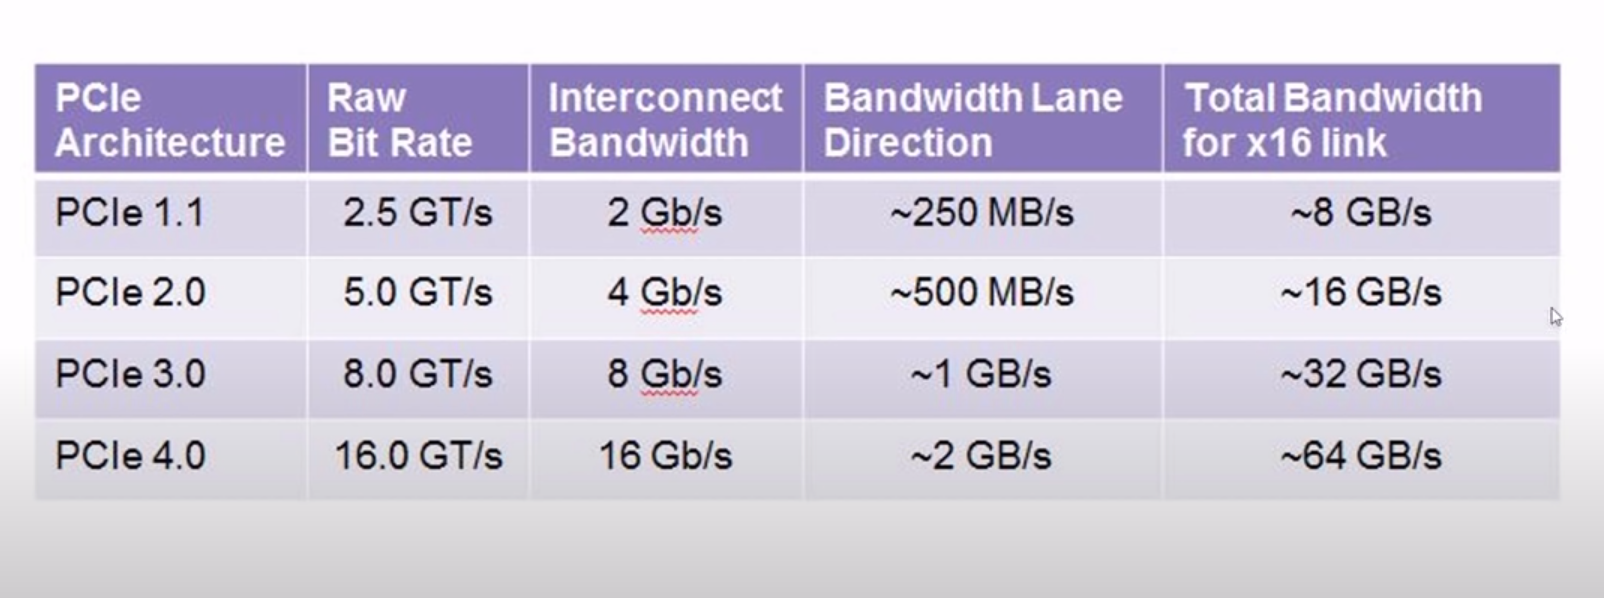
\includegraphics[width=5in]{images/PCIeSpeeds.png}
		\caption{PCIe Speeds}
		\label{PCIeSpeeds}
	\end{center}
\end{figure}

\subsection{PCIe features}

\begin{itemize}
	\item PCIe is a point to point system. So one can have a master and slave similar to RS-232.
    \item PCIe is a serial bus, which means it requires much fewer pins than a parallel bus.
    \item PCIe is also scalable and allows for lane aggregation. This means that if a single lane can transfer 2GB/s another lane can transfer 4GB/s, thus scaling up the bandwidth two times. 
    \item PCIe is also packet based transaction protocol similar to ethernet and it uses the same memoryIO configuration address space as PCI. which means it's backward compatible with PCI.
    \item PCIe also has improved data integrity and error handling.
\end{itemize}


\subsection{PCI connector}

PCI Express comes commonly in two sizes: The 1 line and the 16 line. The 1 line is used for regular boards and 16 lines are useful graphic cards. The 1 link connect has 36 contacts arranged in two rows of 18 contacts. Out of the 36 contacts, only six are useful to transfer data. The rest are power lines as well as auxiliary signals.\\
The six function opens are use in three pairs. The first pair is called REFCLK, which is the reference clock pair. The Second pair is your PER, which is a received pair. And the last one is a transmit pair, which is called PET.\\
So the pairs are often referred to as differential pairs because a signal from a pair carries the same signal, but with one inverted from the other. The reason for using differential pairs is mainly for reliability of transmission.


\subsection{PCIe clock recovery}

At speeds starting at 2.5 GHz, the point to point architecture is still a challenge to get working because the duration of each part is so short. The timing jitter, which is the timing, uncertainty surrounding the arrival each but becomes a problem. And even if each signal pair had an associated clock pair transferred along with it the clockpair also be subjected to timing jitter. So instead, a new technique called clock recovery is used.\\
Basically for each signal pair, a pair receiver looks at the signal transitions a bit zero,followed by a bit one or vice versa from which it can infer the position of the surrounding bits.

\subsubsection{8b/10b encoding}
So one problem is that many successive bits are transmitted with the same value. Like a lot of zeros or a lot of ones and also no signal transition is seen.\\
So extra transmit transmitted to ensure that the signal transitions are not too far apart, which synchronizes the clock recovery mechanism. The extra bits are sent using a scheme called 8b/10b encoding, so that for each 8 bits of useful data inputs are actually transmitteda 20 percent overhead, basically in a specific way that guarantees enough signal transitions.\\
Unfortunately, that also means that for 2.5 gigahertz we only have 250 mbps of useful bandwidth per pair, instead of the three 312 mbps, which would usually get without encoding overhead.\\\\
Differential pair lanes:\\
Advantages\\
1. It is more immune to external interference's like EMF or electromagnetic fields.\\
2. It can operate at low voltages. Lower voltages also mean lower power consumption and thus help for Clock recovery to get a more precise signal transition. \\\\
Disadvantage\\
1. It takes twice as many wires to transmit one signal.\\
\subsubsection{Packetized transactions}

PCI Express is a serial bus. Hence, from a computer's perspective, it is a conventional bus where read and write transactions can be achieved. The trick is that all operations are packetized. \\\\
Let us assume the CPU wants to write some data to the device. It folds the order to the PCI Express bridge, which generates a packet. The packet contains the address and data to be written and is forwarded serially to the targeted device. And thus the device depacketizes the data and executes it.\\\\
While reading the data, the bridge forwards packet to the targeted device which now has to execute to read, create a return packet and send it to the bridge.

\subsection{PCIe Stack}

As packets are transmitted at very high speed, they have to be deserialized, assembled, decoded (8b/10b encoding) at destination,  interleaved if multiple lines are used and then checked against line corruption, which means using CRC checks.\\\\
Most of the complex functions mentioned above are handled by the PCIExpress stack. PCIExpress stack is composed of three layers Physical layer, Datalink layer, and Transition layer.

\begin{figure}[H]
	\begin{center}
		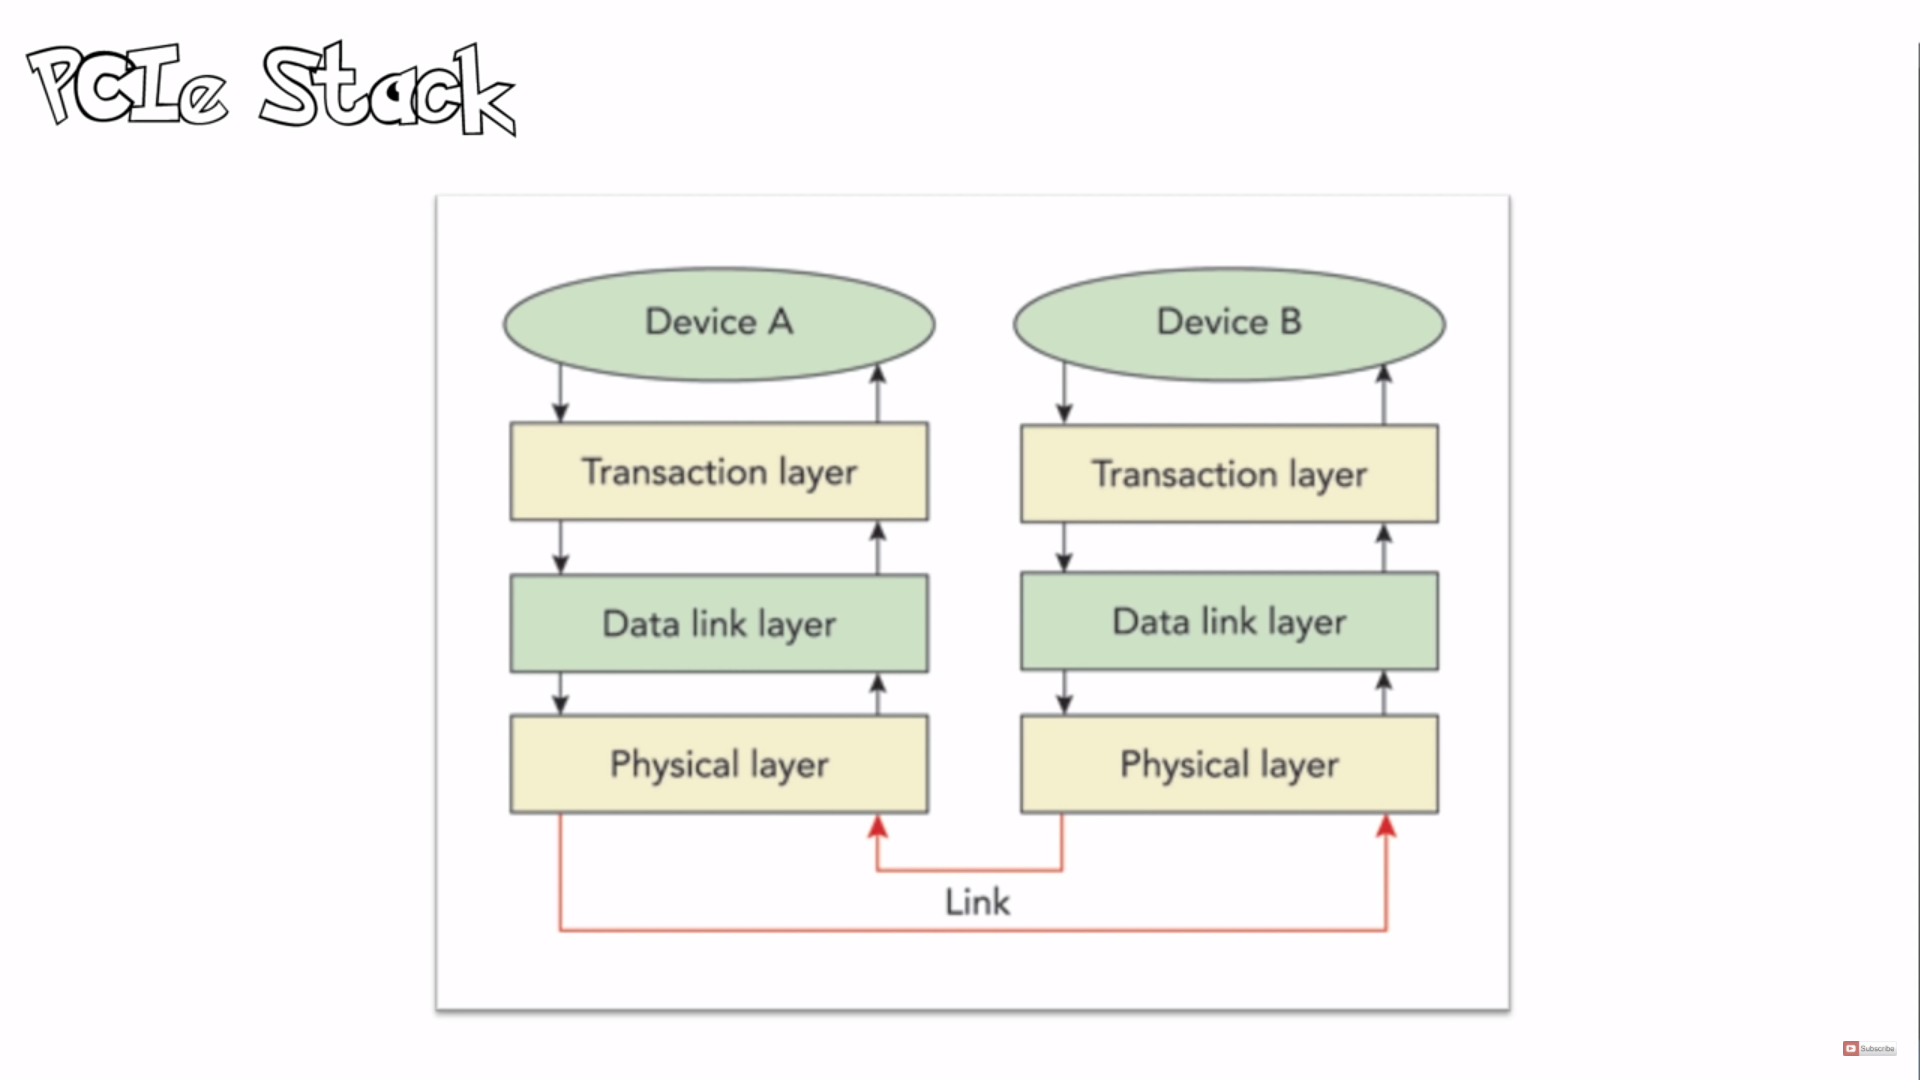
\includegraphics[width=5in]{images/PCIeStack.png}
		\caption{PCIe Stack}
		\label{PCIeStack}
	\end{center}
\end{figure}

PCI Express FPGA core usually which is a combination of the hard and soft core. This handles all the complexity. So as the user end, one only has to work in the transaction layer.\\
\begin{itemize}
	\item Physical layer comprises of pins toggling, 8b/10b encoding,decoding, 
link assembly and disassembly.
    \item Data link layer checks the data integrity, checks CRC (cyclic redundancy check).
    \item PCIe transaction layer receive packets. The packet lengths are always multiples of 32 ("double word") as they arrive on the 32bit bus. Transaction layer accept packets and issues packets as it's main task. The packets are structured in a specific format called the Transaction Layer Packets "TLPs". TLPs contain a header and a data payload. The header contains 3 or 4 double words where as the data payload can range from 0 to 1023 double words, and even up to 4096 double words in latest generations.
\end{itemize}


